% simple.tex – Un exemple d'article simple pour illustrer la structure d'un document.
\documentclass{article}
\usepackage[french]{babel}
\usepackage[T1]{fontenc}
\usepackage{times}
\usepackage[backend=biber, style=authoryear,sorting=nty]{biblatex}
\usepackage{graphicx}

\graphicspath{{./figures}}
\addbibresource{bibliography.bib}

\title{RAG et implementations possibles}
\author{Anas Lahrouchi, Pradityo WicaKsono\\
   UFR IM2AG,\\
   Université de Grenoble Alpes,\\
   \texttt{Anas.Lahrouchi@etu.univ-grenoble-alpes.fr}}
\date{\today}


\begin{document}
\maketitle
\newpage

\section{Pourquoi a-t-on besoin d'un RAG?}

\subsection{C'est quoi un RAG?}

Les grands modèles de langage (LLM) peuvent être inconsistant. En général, ils ont des réponses qui correspondent exactement aux requêtes, 
parfois ils ont des réponses qui sont compléments incorrects, on appelle ces cas-là des "hallucinations". Ce problème provient 
du fait que le dataset d'entrainement du LLM n'est pas à jour et que le modèle ne sait pas s'il a une réponse ou non.

Retreival Augmented Generation (RAG) est un Framework d'intelligence artificielle qui vise à améliorer la qualité des réponses générées par les LLM 
en fournissant un contexte se basant sur des données externes avec chaque requête pour compléter la représentation internes des informations du LLM. 
Implémenter RAG dans un système LLM a deux bénéfices : il assure que le modèle à accès aux faits actuelles les plus précises et que l'utilisateur a 
accès aux sources du modèle assurant ainsi que la validité et la précision des réponses peuvent être vérifier \footcite{ibmragarticle23}.

\subsection{Comment fonctionne un LLM avec un RAG?}


Un RAG prend comme entrée la requête de l'utilisateur, il récupère un ensemble de documents pertinents et justificatifs depuis une base de connaissance. 
Les documents sont ensuite concaténés et fournis avec la requête en tant que contexte à LLM, ce dernier génère la réponse à la requête de l'utilisateur\footcite{heikohotz23}.

\begin{figure}[h]
   \begin{center}
   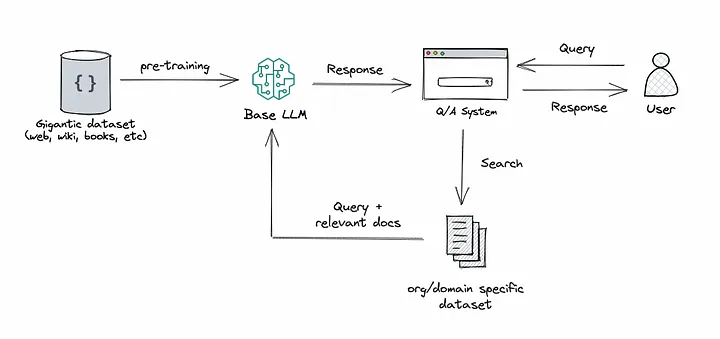
\includegraphics[width=\textwidth]{rag-simple-explanation.png}
   \caption{une explication simple du Framework RAG}
   \end{center}
   \label{explicationsimplerag}
\end{figure}


\section{Quelles sont les implementations possibles de ce concept?}

Le Framework RAG a différentes implémentations, ca dépend des exigences et contraintes de l'application en question. 
Durant ce travail, Nous discutrons les implémentations suivantes:

\subsection{RAG basée sur une récupération par mot clés}

La première approche que nous allons discuter, la recherche par mots clés ou son extension la recherche par texte, est 
utilisée dans différents systèmes informatiques, tel que les navigateurs internet, les sites e-Commerce, les systèmes de gestion de fichiers. 
Il existe plusieurs implémentations de la recherche par mots clés, nous allons voir le cas du système open-source appelé ElasticSearch. 
ElasticSearch est un moteur de recherche et d'analyse distribué qui a comme noyau Apache Lucene développé en Java. 
Il nous permet de stocker, chercher et analyser des gros volumes de data rapidement et en temps réel. Alors comment fonctionne Elastic search? 

\subsubsection{les stuctures de données utilisées}

\textbf{Les document JSON} sont est l'unité informatique basique d'ElasticSearch. Un document peut être comparé à une ligne dans une base relationnelle.
Chaque Document a un identifiant unique et un type de donnée décrivant son contenu. 

\textbf{Un index} est une collection de documents aux caractéristique similaires, il s'agit du plus haut niveau d'entité sur laquelle on peut effectuer des requêtes. ElasticSearch   
utilise \textbf{des index inversés}. Ce mécanisme est à la source du fonctionnement de tous les moteurs de recherche, et associe un mapping du contenu à son emplacement dans 
un document ou un ensemble de documents. Cette structure de données hashmap-like permet de se diriger d’un mot vers un document\footcite{Gopalakrishnan23}. 

\subsubsection{Un système distibué}

\begin{figure}[h]
   \begin{center}
   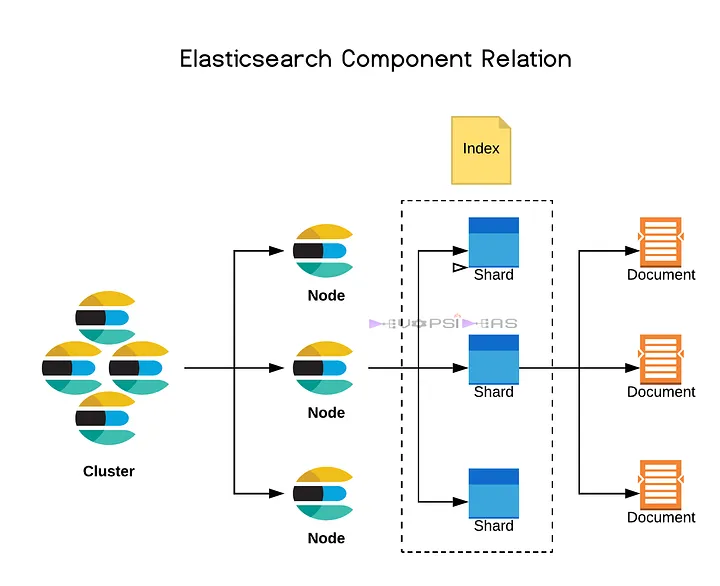
\includegraphics[width=\textwidth]{Elasticsearch-component-relation.png}
   \caption{Les composants du syste ElasticSearch\footcite{DevopsIdeas22}}
   \end{center}
   \label{explicationsimplerag}
\end{figure}

Un cluster est constitué d'un ou plusieurs instances de node connectées.
Un node est un serveur qui appartient à un cluster, il stock les données, il les indexe et il effectue des recherches.
Un index peut etre sous-divisé en fragment(shards), chaque fragment est un index indépendant et pleinement fonctionnel 
pouvant être hébergé sur n’importe quel noeud au sein d’un cluster\footcite{Gopalakrishnan23}.


\newpage

\printbibliography

\listoffigures

\end{document}